\documentclass[tikz, preview]{standalone}

\usepackage{amsfonts, amsthm, amssymb, amsmath, stmaryrd, etoolbox}
\usepackage{tikz}
\usetikzlibrary{matrix,arrows}

\begin{document}
\[
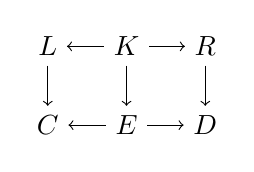
\begin{tikzpicture}
\node (L) at (-1,1) {$L$};
\node (K) at (0,1) {$K$};
\node (R) at (1,1) {$R$};
\node (C) at (-1,0) {$C$};
\node (E) at (0,0) {$E$};
\node (D) at (1,0) {$D$};
%
\draw [->] (K) edge (L);
\draw [->] (K) edge (E);
\draw [->] (K) edge (R);
\draw [->] (E) edge (C);
\draw [->] (E) edge (D);
\draw [->] (L) edge (C);
\draw [->] (R) edge (D);
\end{tikzpicture}
\]
\end{document}
